\documentclass{beamer}
% \usetheme{metropolis}

\usepackage{graphicx}
\usepackage{tikz}
\usepackage{caption}
\usepackage{adjustbox}
\usepackage{listings}
\usepackage{wrapfig}
\usepackage{color}
\usepackage{listings}
\usepackage{pgfpages}
\usepackage{msc}
% \setbeameroption{show notes on second screen=right}

\usetikzlibrary{automata,positioning,shapes,snakes}
\usetikzlibrary{calc,matrix,arrows,automata,decorations.pathmorphing}
\usetikzlibrary{shapes.geometric,arrows.meta}
\pgfmathtruncatemacro\distance{1}

\addtobeamertemplate{navigation symbols}{}{%
    \usebeamerfont{footline}%
    \usebeamercolor[fg]{footline}%
    \hspace{1em}%
    \insertframenumber/\inserttotalframenumber
}

\setbeamercolor{footline}{fg=blue}
\setbeamerfont{footline}{series=\bfseries}

\tikzset{
    mylabel/.style={
    font=\tiny,
    sloped,
    above
  }
}

\lstset{language=erlang, basicstyle=\sffamily\footnotesize,
  keywordstyle=\color{blue}, numberstyle=\tiny, numbers=none,
  showspaces=false, showstringspaces=false, frame=tL, mathescape=true,
  backgroundcolor=\color{black!5}, morekeywords={send, to, from} }


\title{On the implementability of Global Types}
\author{\textbf{Gabriele Genovese}\\Supervisor: Cinzia Di Giusto}
\date{4 July 2025}

\titlegraphic{
\includegraphics[width=3cm]{unica}\hspace*{4.75cm}~%
   
\includegraphics[width=2cm]{i3s}
}


\begin{document}

\maketitle
\note{
	Good morning, everyone. I'm Gabriele Genovese.
}


% slide 1
\begin{frame}{Formal Distributed Systems}
	\begin{itemize}
		\item Abstractions used to simplify the study and development:
		      \begin{itemize}
			      \item Global Types
			      \item Message Sequence Charts (MSC)
		      \end{itemize}
		      \bigskip
		\item Useful for proving various properties
	\end{itemize}
\end{frame}

\newcommand{\marrow}[3]{#1\xrightarrow{#3}#2}
\newcommand{\gtlabel}[3]{\marrow{#1}{#2}{#3}}
\begin{frame}{Global Types}

	\begin{itemize}
		\item Description of a \textbf{global} behavior of a communication system.

		      \bigskip

		\item Automaton: visual representation of the global type.
	\end{itemize}

	\bigskip

	\begin{center}
		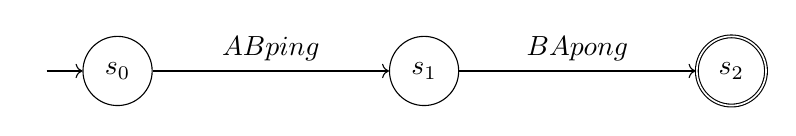
\begin{tikzpicture}[node distance=3cm, auto]
			\node[state, initial, initial text={}] (s0) {$s_0$};
			\node[state] (s1) [right=of s0] {$s_1$};
			\node[state,accepting] (s2) [right=of s1] {$s_2$};

			\draw[->] (s0) -- node[above,sloped]{$\gtlabel{A}{B}{ping}$} (s1);
			\draw[->] (s1) -- node[above,sloped]{$\gtlabel{B}{A}{pong}$} (s2);
		\end{tikzpicture}
	\end{center}
\end{frame}

\begin{frame}{Local type}
	\begin{itemize}
		\item Point of view of a participant
		\item Typically obtained with a \textit{projection} operation
	\end{itemize}

	\bigskip

	\begin{center}
		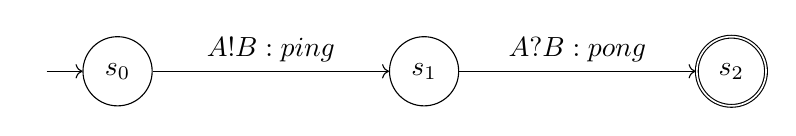
\begin{tikzpicture}[node distance=3cm, auto]
			\node[state, initial, initial text={}] (s0) {$s_0$};
			\node[state] (s1) [right=of s0] {$s_1$};
			\node[state,accepting] (s2) [right=of s1] {$s_2$};

			\draw[->] (s0) -- node[above,sloped]{$A!B:ping$} (s1);
			\draw[->] (s1) -- node[above,sloped]{$A?B:pong$} (s2);
		\end{tikzpicture}
	\end{center}

	\begin{center}
		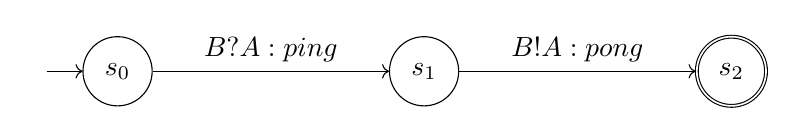
\begin{tikzpicture}[node distance=3cm, auto]
			\node[state, initial, initial text={}] (s0) {$s_0$};
			\node[state] (s1) [right=of s0] {$s_1$};
			\node[state,accepting] (s2) [right=of s1] {$s_2$};

			\draw[->] (s0) -- node[above,sloped]{$B?A:ping$} (s1);
			\draw[->] (s1) -- node[above,sloped]{$B!A:pong$} (s2);
		\end{tikzpicture}
	\end{center}
\end{frame}

\begin{frame}{Example}
	Message Queuing Telemetry Transport (MQTT) protocol with two clients.
	\begin{center}
		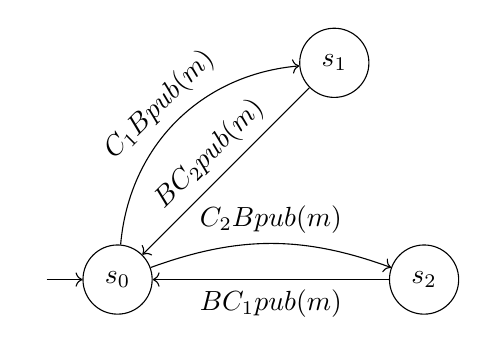
\begin{tikzpicture}[node distance=3cm, auto]
			\node[state, initial, initial text={}] (s0) {$s_0$};
			\node[state] (s1) [above right=of s0] {$s_1$};
			\node[state] (s2) [right=of s0] {$s_2$};

			\draw[->, bend left=40] (s0) to node[above,sloped]{$\gtlabel{C_1}{B}{pub(m)}$}(s1);
			\draw[->] (s1) to node[above,sloped] {$\gtlabel{B}{C_2}{pub(m)}$} (s0);

			\draw[->, bend left=20] (s0) to node[above,sloped]{$\gtlabel{C_2}{B}{pub(m)}$}(s2);
			\draw[->] (s2) -- node[below,sloped]{$\gtlabel{B}{C_1}{pub(m)}$} (s0);
		\end{tikzpicture}
	\end{center}
\end{frame}

\newcommand{\arrmess}[3]{%
	$#1 \xleftrightarrow{#3} #2$
}

\newcommand{\syncmscmess}[3]{%
	\mess{#1}{#2}{#3}%
	\mess{}{#3}{#2}%
	\nextlevel
}

\newcommand{\asyncmscmess}[3]{%
	\mess{#1}{#2}{#3}%
	\nextlevel
}

\begin{frame}[fragile]{Message Sequence Charts (MSC)}
	Diagrams used to represent traces of a behavior of the system.

	\bigskip

	% \hspace{-2em}
	\begin{minipage}{\textwidth}%0.45\textwidth}
		\centering
		\begin{msc}[draw frame=none, draw head=none, msc keyword=, head height=0px, label distance=0.5ex, foot height=0px, foot distance=0px]{}
			\declinst{P1}{P1}{}
			\declinst{P2}{P2}{}
			\declinst{P3}{P3}{}

			\asyncmscmess{$m_1$}{P1}{P2}
			\asyncmscmess{$m_2$}{P2}{P3}
		\end{msc}
	\end{minipage}
	% \hspace{0.1\textwidth}
	% \begin{minipage}{0.45\textwidth}
	% 	\centering
	% 	\begin{msc}[draw frame=none, draw head=none, msc keyword=, head height=0px, label distance=0.5ex, foot height=0px, foot distance=0px]{}
	% 		\declinst{P1}{P1}{}
	% 		\declinst{P2}{P2}{}

	% 		\mess{$m_1$}{P1}{P2}[1]
	% 		\mess{$m_2$}{P2}{P1}[3]
	% 	\end{msc}
	% \end{minipage}
	% descrive gli eventi send and receive
	\begin{center}
		Events: \verb|send m1, receive m1, send m2, receive m2|
	\end{center}
\end{frame}

\begin{frame}{The implementability problem}
	Property to guarantee: \textbf{respectfulness} the behavior described.

	\bigskip

	Does the implementation of a system \textbf{respects}
	the behavior described?
\end{frame}

\begin{frame}[fragile]{Example}

	\begin{itemize}
		\item 4 participants: $A, B, C, D$
		\item 4 messages: $x, y, z, w$
		\item Specification description:
	\end{itemize}

	\bigskip

	\begin{lstlisting}
A send B either message x or y.

if A send B message x,
    then C send B message z.

if A send B message y,
    then C send B message w.
    \end{lstlisting}
\end{frame}

%% estendere il comportamento
\begin{frame}{Example's global type}
	% This graph is \textbf{not} implementable because $c$ doesn't know what $b$ received.
	\begin{center}
		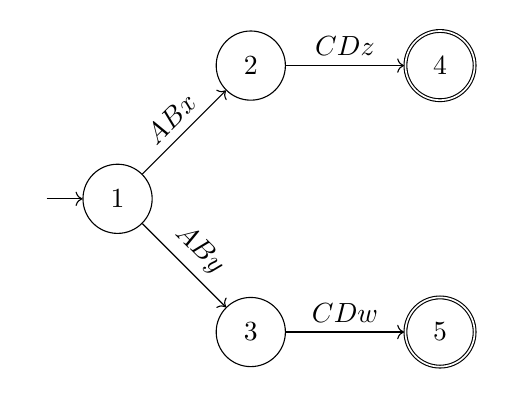
\begin{tikzpicture}[node distance=1.5cm, auto]
			\node[state, initial, initial text={}] (s0) {1};
			\node[state] (s1) [above right=of s0] {2};
			\node[state] (s2) [below right=of s0] {3};
			\node[state,accepting] (s3) [right=of s1] {4};
			\node[state,accepting] (s4) [right=of s2] {5};

			\draw[->] (s0) to node[above,sloped]{$\gtlabel{A}{B}{x}$}(s1);
			\draw[->] (s0) to node[above,sloped]{$\gtlabel{A}{B}{y}$}(s2);
			\draw[->] (s1) to node[above,sloped]{$\gtlabel{C}{D}{z}$}(s3);
			\draw[->] (s2) to node[above,sloped]{$\gtlabel{C}{D}{w}$}(s4);

		\end{tikzpicture}
	\end{center}
\end{frame}

\begin{frame}{Example's global type}
	This Global Type is {\color{red}\textbf{not}} implementable because $c$ doesn't know what $b$ received.
	\begin{center}
		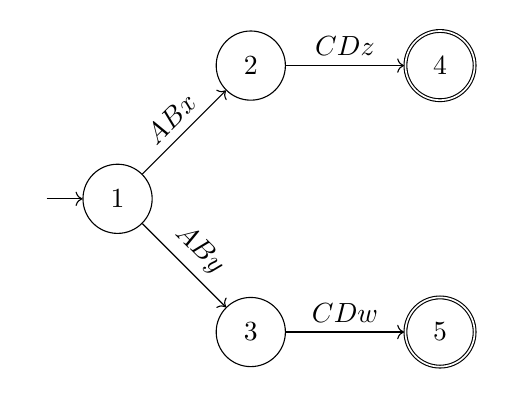
\begin{tikzpicture}[node distance=1.5cm, auto]
			\node[state, initial, initial text={}] (s0) {1};
			\node[state] (s1) [above right=of s0] {2};
			\node[state] (s2) [below right=of s0] {3};
			\node[state,accepting] (s3) [right=of s1] {4};
			\node[state,accepting] (s4) [right=of s2] {5};

			\draw[->] (s0) to node[above,sloped]{$\gtlabel{A}{B}{x}$}(s1);
			\draw[->] (s0) to node[above,sloped]{$\gtlabel{A}{B}{y}$}(s2);
			\draw[->] (s1) to node[above,sloped]{$\gtlabel{C}{D}{z}$}(s3);
			\draw[->] (s2) to node[above,sloped]{$\gtlabel{C}{D}{w}$}(s4);

		\end{tikzpicture}
	\end{center}
\end{frame}


\tikzstyle{box} = [rectangle, rounded corners, draw=blue!60, fill=blue!10, thick,
text width=7.5em, text centered, minimum height=2em]



\begin{frame}{Reduction to sync}
	A global type $G$ is implementable in \textbf{p2p} iff:
	\begin{enumerate}
		\item $L_{\text{p2p}}(proj(G))$ is a set of sync MSCs;
		\item $proj(G)$ is orphan-free in p2p; % (no message is sent but not received)
		\item $L_{\text{p2p}}(proj(G))$ is deadlock-free
		\item $G$ is implementable in sync
	\end{enumerate}
\end{frame}

% i primi 3 punti sono decidibili
\begin{frame}{Reduction to sync}
	A global type $G$ is implementable in \textbf{p2p} iff:
	\begin{enumerate}
		\item $L_{\text{p2p}}(proj(G))$ is a set of sync MSCs;
		\item $proj(G)$ is orphan-free in p2p; % (no message is sent but not received)
		\item $L_{\text{p2p}}(proj(G))$ is deadlock-free
		\item \textbf{$G$ is implementable in sync} \scalebox{1.5}{{\color{red}$\longleftarrow$}}
	\end{enumerate}
\end{frame}

\begin{frame}{My contribution}
	Extension of a proof to a general framework:

	\bigskip

	\begin{itemize}
		\item Original theorem: checking implementability for bounded
		      MSCs is undecidable

		      \bigskip

		\item \textbf{Now}: checking implementability for sync-global
		      types is undecidable

		      \bigskip

		\item Proof: by reduction to the PCP problem
	\end{itemize}
\end{frame}


\begin{frame}{Post Correspondance Problem (PCP)}
	Given a set of tiles, find an ordering such that the
	strings formed by the top and bottom halves are equal.

	\begin{center}
		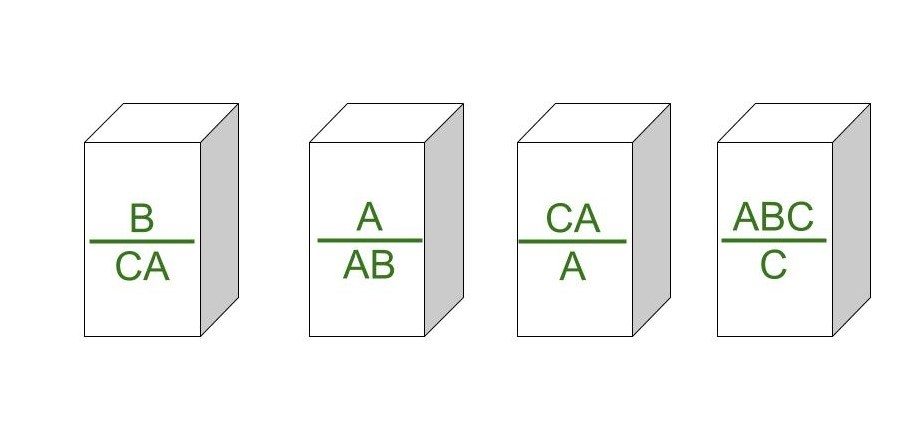
\includegraphics[width=0.7\textwidth]{pcp.jpg}
	\end{center}

	% Possible solution: 2, 1, 3!
\end{frame}

% generalizzare p2p ad altri
\begin{frame}[fragile]{Future work}
	\begin{itemize}
		\item Extend existing results using the \verb|com|-general framework

		      \bigskip

		\item Extend and adapt a model checking tool to the \verb|com|-general framework
	\end{itemize}
\end{frame}

\begin{frame}{Reduction to sync}
	A global type $G$ is implementable in \textbf{p2p} iff:
	\begin{enumerate}
		\item $L_{\text{p2p}}(proj(G))$ is a set of sync MSCs;
		\item $proj(G)$ is orphan-free in p2p; % (no message is sent but not received)
		\item $L_{\text{p2p}}(proj(G))$ is deadlock-free
		\item $G$ is implementable in sync
	\end{enumerate}
\end{frame}

\begin{frame}{Hierarchy of communication models}
	More interesting: async, p2p, mb (mailbox), rsc (sync).

	\bigskip

	\begin{center}
		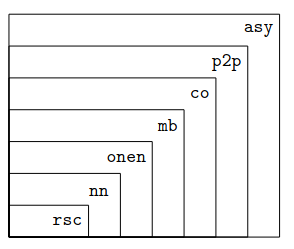
\includegraphics[width=0.3\textwidth]{hierarchy.png}
	\end{center}
	\bigskip
	\begin{center}
		% {\color{red}
		% 	\textbf{Create a theory that generalyze communication models}
		% }
	\end{center}
\end{frame}

\begin{frame}{State of the art}
	The study about implementability can be summarized in:

	\bigskip

	\begin{center}
		% spendere più parole su standard:
		% la sintassi degli MPST permette l'implementazione
		\begin{tikzpicture}[node distance=0.64cm]
			\node (ind) [box] {Standard};
			\node (sci) [box, right=1cm of ind] {Semantic};
			\node (desc1) [box, below=of ind] {By contruction, easy and efficient\\E.g. MPST};
			\node (desc3) [box, below=of sci] {More foundamental: what renders a global type implementable?};
			\draw[->] (ind) -- (desc1);
			\draw[->] (sci) -- (desc3);
			\draw[->] (desc1) -- (ind);
			\draw[->] (desc3) -- (sci);
			\draw[->] (ind) -- (sci);
		\end{tikzpicture}
	\end{center}
\end{frame}

\begin{frame}[fragile]{Our approach: semantic}
	\begin{itemize}
		\item What render a specification implementable?
		\item What is the limit? Why syntactical constraints works?
		\item \textbf{Aim}: Extend existing results and generalize to
		      different communication models
		      % \begin{itemize}
		      %  \item \verb|p2p|
		      %  \item \verb|mailbox|
		      %  \item \verb|sync|
		      % \end{itemize}
	\end{itemize}
\end{frame}

\begin{frame}[fragile]{Conclusion \& Future work}
	Summerize:

	\bigskip

	\begin{itemize}
		\item Study of the implementability problem for global types

		      \bigskip

		\item Proof of undecidability

		      \bigskip

		\item Extend existing results and tool using the \verb|com|-general framework
	\end{itemize}
\end{frame}

\begin{frame}{Other activities}
	\begin{itemize}
		\item Partecipation at an International \textbf{Conference}, DisCoTec
		\item Obtained a \textbf{PhD grant} (DS4H)
		\item Future participation to a \textbf{Summer School} in Software Verification in Edimburgh
	\end{itemize}
	\bigskip
	\begin{center}
		\Large Thanks! Questions?
	\end{center}
\end{frame}

% \begin{frame}
% 	\begin{center}
% 		\Large Thanks! Questions?
% 	\end{center}
% \end{frame}


\end{document}
